\section{Examples}\label{sec:examples}


\subsection{Concurrent Spanning Tree}\label{subsec:CST-example}

Programs manipulating arbitrary graphs present a
significant challenge for compositional verification: because of deep,
\emph{unspecified} sharing between different components of a graph,
changes to one subgraph may affect other subgraphs which may point
into it. This makes it hard to reason about updates to each subgraph
in isolation. In a concurrent setting, this difficulty compounds with
the fact that threads working on different parts of the graph may
affect each other in ways that are difficult to reason about locally
to each subgraph. We now demonstrate on a concurrent spanning tree
example that \colosl may be just the tool needed in this case, as it
naturally deals with arbitrary overlapping views of the shared state,
and allows one to tailor interferences to a given subjective view,
achieving local reasoning about the shared state for this challenging program.

Our example, presented in \fig\ref{fig:conSpanningTree}, operates on a
\emph{directed binary graph} (henceforth simply \emph{graph}): 
that is,  a directed graph where each node has at most two
successors, called its left and right children. The program concurrently computes an
in-place spanning tree of the graph (i.e.\ a tree that covers
all nodes of the graphs from a given root), as follows:
each time a new node is encountered, two new threads are created that
each prune the edges of its left and right children recursively. A
mark bit is associated with each node to keep track of which nodes  have
already been visited. Each thread returns whether it marked the node
it was called on itself or whether somebody else did. In the latter case,
the parent thread removes the link from its own root node to the
corresponding child. Intuitively, it is allowed to do so because the
child has already been  reached via some other path in the graph since it was marked by another thread.

%% marking the vertices to keep track of those already visited; the
%% return value b records the outcome of marking with \li{b}$=1$ when the
%% top node $x$ is unmarked (not visited yet) and \li{b}$=0$
%% otherwise. Assuming that the root vertex $x$ is unmarked initially,
%% the algorithm continues by first marking $x$ and subsequently spanning
%% the left and right subgraphs concurrently. When the top node of the
%% left subgraph is already marked (\li{!b1}), the edge from $x$ into it
%% is replaced by a null pointer. This corresponds to the case where the
%% node has already been visited by another thread and is thus reachable
%% from the root; \emph{mutatis mutandis} for the right subgraph.

We will prove that, given a shared graph as input, the program always
returns a tree, i.e.\ all sharing and cycles have been
appropriately removed. Pleasingly, the \colosl specification captures just the subgraph
manipulated by the thread, instead of the whole graph. 
%Because of
%arbitrary sharing between the two, a proof using a more global specification would be
%unpleasant indeed. 
%However, we do not establish that the final tree
%indeed spans the original graph. The reason it does is subtle indeed,
%as are the invariants required, but in ways unrelated to our main
%issue, which is to provide tight specifications for each thread.

To reason about this program, following~\cite{ramification} we use two representations of graphs. The
first is a mathematical representation $\gamma = (V, E)$ where $V$ is
a finite set of vertices and $E: V \rightarrow (V \uplus
\{\li{null}\}) \times (V \uplus \{\li{null}\})$ is a function
associating each vertex with at most two successors, where \li{null}
denotes the absence of a child.  We write $n \in \gamma$
for $n \in V$, $\gamma(n)$ for $E(n)$ which also assumes $n \in \gamma$, $n\leadsto_\gamma n'$ for
$n'\in \gamma(n)$, and $\leadsto^{\ast}_\gamma$ for the reflexive and
transitive closure of $\leadsto_\gamma$.

Mathematical graphs are connected to their in-memory representations
by a predicate $\graph{x}{\gamma}$ shown in \fig~\ref{fig:globalCST}, denoting a spatial
(in-heap) graph rooted at address $x$ corresponding to the
mathematical graph $\gamma$. This predicate uses the overlapping conjunction to account
for potential sharing between the left and right children and for potential
cycles in the graph.
%Such an action is allowed by a
%\emph{marking} capability of the form $\markT{n}{e}$ where $n$ denotes
%the vertex (address) and $e$ the edge via which vertex $n$ is visited.
%Thus owning an unmarked vertex grants the right to visit and mark its
%unmarked children, and the capabilities owned on the same node by
%multiple threads do not clash since they would have gotten to that
%node via different paths which yield different capabilities. For
%instance, the capabilities associated with marking of vertex $z$ in
%\fig\ref{fig:graphAndTree} are $\markT{z}{y.r}$ and
%$\markT{z}{w.l}$. Note that the parameterisation of our actions are
%merely a notational convenience and can be substituted for their full
%definitions. In order to account for the ability to mark the root
%vertex $x$ of a graph, we introduce a logical (virtual) root edge
%$\rootEdge$ into $x$ as depicted in \fig\ref{fig:graphAndTree}
%together with its associated marking capability
%$\markT{x}{\rootEdge}$. 
%% Note that the two subgraphs and vertex $x$ are combined by
%% the overlapping conjunction $\sepish$ since the graph can be cyclic
%% and each node may be reachable via more than one path.
%
%\begin{wrapfigure}[8]{r}{0.25\textwidth}
%	\centering
%	\begin{tabular}{|c |}
%		\hline
%			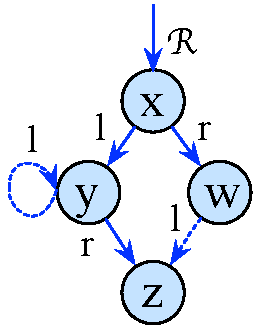
\includegraphics[scale=0.27]{Sections/Examples/Images/graph.pdf} \\
%		\hline
%	\end{tabular}
%\caption{A graph.}
%\label{fig:graphAndTree}
%\end{wrapfigure}
%%%
Each vertex is represented as three consecutive cells in the heap
tracking the mark bit and the addresses of the left and right
subgraphs. We write $\cell{x}{m, l, r}$ for $\cell{x}{m} *
\cell{x+1}{l} * \cell{x+2}{r}$, and $x.l$ and $x.r$ for $x+1$ and
$x+2$, respectively. When vertex $x$ is in the unmarked state
$\unmarked{x}{l}{r}$, the whole cell $\cell{x}{0,l,r}$ resides in the
shared state. In the marked state $\marked{x}$, only $\cell{x}{1}$ is
owned. In both cases, the shared state also contains the left and
right subgraphs represented by $\G{l}{\gamma}$ and $\G{r}{\gamma}$.

To understand the difference in ownership between $\unmarked{x}{l}{r}$ and $\marked{x}$, let us look at the interference associated
with the graph, which is the union of interferences pertaining each
vertex in the graph. For each vertex $n \in \gamma$, the only
permitted action is that of marking $n$. (For simplicity, this action
does not require any capability.)  When changing the mark field of $n$
from $0$ to $1$, the current thread also claims ownership of its left
and right pointers. Indeed, we observe that other threads need not
access the children of $n$ once they see that it has already been
marked. The atomic \li{CAS} (compare-and-swap) instruction prevents
two threads from concurrently marking the same node and claiming ownership
of the same resource.
%% The shared state contains node $x$ which can
%% be either unmarked ($\unmarked{x}{l}{r}$) or marked ($\marked{x}$); as
%% well as the left and right subgraphs represented recursively by
%% $\G{l}{\gamma}$ and $\G{r}{\gamma}$.

%which can be carried out by any of the marking capabilities associated with node $n$ ($\markT{n}{-}$). 
%\begin{figure}
% %\centering
%%  \hspace*{0.2cm}
%  \begin{minipage}{0.98\linewidth}
%    \begin{tabular}{| c | l |}
%    \hline	
%    %\hspace*{-0.4cm}
%    \begin{subfigure}[b]{0.14\textwidth}			
%      \centering	
%      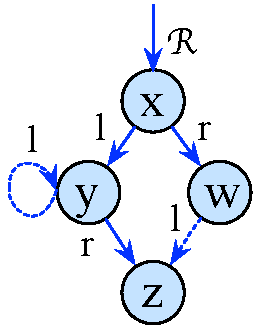
\includegraphics[scale=0.35]{Sections/Examples/Images/graph.pdf}\vspace*{5pt}\\
%    \caption{}
%    \label{fig:graphAndTree}
%    \end{subfigure}
%    &
%    \begin{subfigure}[b]{0.86\textwidth}	\vspace{5pt}		
%    $\begin{array}{@{\hspace{10pt}} r @{\hspace*{2pt}} l}
%			\graph{x}{\gamma} \eqdef & \left[\markT{x}{\rootEdge}\right] * \shared{\G{x}{\gamma}}{I_\gamma} \hspace*{0.5cm} I_\gamma \eqdef \bigcup\limits_{n \in \gamma}I(n)\\
%%	
%			\G{x}{\gamma} \eqdef & (x = \li{null} \land \emp) \lor x \in \gamma \land \exsts{l, r} \gamma(x) = (l, r) \\
%			& \land \left( \unmarked{x}{l}{r} \lor \marked{x}\right) \sepish \G{l}{\gamma} \sepish \G{r}{\gamma}\\
%%
%			\unmarked{x}{l}{r} \eqdef & \cell{x}{0, l, r} * \left[\markT{l}{x.l}\right] * \left[\markT{r}{x.r} \right]
%			\qquad
%			\marked{x} \eqdef  \cell{x}{1}\\
%%
%			I(n) \eqdef & \left\{ \markT{n}{-}: \exsts{l, r} \unmarked{n}{l}{r} \swap \marked{n}\right\}
%		\end{array}
%		$
%		 \caption{}
%    \label{fig:globalCST}
%    \end{subfigure}\\
%    \hline
%    \end{tabular}
%    %\caption{Abstract (de)allocation in SSL}
%    \label{fig:graph-and-globalCST}	
%  \end{minipage}
%\caption{A binary graph (left); global specification of the graph predicate (right).}
%\end{figure}
%
\begin{figure}
  \hrule\vspace{-5pt}
  \begin{mathpar}
  \graph{x}{\gamma} \eqdef
  \shared{\G{x}{\gamma}}{I_\gamma}
  \qquad
  I_\gamma \eqdef \bigcup_{n \in \gamma}I(n)
  \qquad
  I(n) \eqdef \left\{ [\emptyset]: \exsts{l, r} \unmarked{n}{l}{r}
  \swap \marked{n}\right\}
  \vspace{-15pt}
  \end{mathpar}
  \begin{align*}
    \G{x}{\gamma} &\eqdef
    \smash{\begin{array}[t]{@{}l@{}}
        (x = \li{null} \land \emp) \lor 
        \exsts{l, r} \gamma(x) = (l, r) \land\null\\
        \left( \unmarked{x}{l}{r} \lor \marked{x}\right) \sepish
        \G{l}{\gamma} \sepish \G{r}{\gamma}
    \end{array}}
    &
    \unmarked{x}{l}{r} &\eqdef \cell{x}{0, l, r} 
    \\
    & 
    &
    \marked{x} &\eqdef  \cell{x}{1}
  \end{align*}
  \hrule
  \caption{Globally-shared graph predicate.}
  \label{fig:globalCST}	
\end{figure}


\begin{figure}
\hrule
\[
\begin{array}{@{}r @{\hspace*{2pt}} l@{}}
	\g{x}{\gamma} \eqdef & (x = \li{null} \land \emp) \lor \exsts{l, r} \gamma(x) = (l, r) \land\null\\
	& \shared{\unmarked{x}{l}{r} \lor \marked{x}}{I(x)} * \g{l}{\gamma} * \g{r}{\gamma}\\
	
	\tr{x}{\gamma} \eqdef & (x = \li{null} \land \emp) \lor (\exsts{l, r} \gamma(x) = (l, r) \land \exsts{l'\!\! \in\! \{l, \li{null}\},r'\!\! \in \!\{r, \li{null}\}}\\
	& \shared{\marked{x}}{I(x)} *
	\cell{x.l}{l'} * \tr{l'}{\gamma} * 
	\cell{x.r}{r'} * \tr{r'}{\gamma})
\end{array}
\]
\hrule
\caption{Locally-shared graph predicate.}
\label{fig:localCST}
\end{figure}

The $\graph{x}{\gamma}$ predicate defined in \fig\ref{fig:globalCST}
is a \emph{global} subjective view of the graph that contains all
vertices and the interference associated with $\gamma$. However, our
spanning tree algorithm operates \emph{locally} as it is called upon
recursively for each node. That is, for each \li{span(n)} call (where
$\li{n} \in \gamma$), the footprint of the call is limited to the
subgraph rooted at $n$. Moreover, in order to reason about the
concurrent recursive calls \li{span(x-}$\!\textgreater$\li{l)
  $\ \mid\mid\ $ span(x-}$\!\textgreater$\li{r)}, we need to
\emph{split} the state into two using $*$, pass each constituent state to the relevant thread and $*$-combine
the resulting states, as required by the
\parRule\ rule. We thus conduct our proof with respect to a
\emph{local} description of the graph, $\g{x}{\gamma}$ as defined in
\fig\ref{fig:localCST}. 
The definition of the $\g{x}{\gamma}$ predicate is similar to that of
$\shared{\G{x}{\gamma}}{I_{\gamma}}$ except that the single view
$\shared{\G{x}{\gamma}}{I_{\gamma}}$ has been broken down into individual
views for each vertex $n$ reachable from $x$. Moreover, the interference
assertion of each local view concerning a vertex $n \in \gamma$ has been shifted
from $I_{\gamma}$ to $I(n)$ so as to reflect only those actions that
affect $n$.  


The $\tr{x}{\gamma}$ predicate, also given in \fig\ref{fig:localCST}, 
represents a \emph{tree}
rooted at $x$, as is standard in separation logic~\cite{rey02}, and
consists, once fully unfolded, of one subjective view for each vertex $n$
reachable from $x$ in
$\gamma$. The assertion of the subjective view for $x$ reflects the
fact that $x$ has been marked, and its left and right pointers
% and the corresponding marking
%capabilities, 
 have been claimed by the marking thread and moved into
its local state. The vertex $l'$ addressed by the left pointer of $x$
corresponds to either the initial value $l$ prior to
marking, or to \li{null} when $l$ has
more than one predecessor and has been marked by another thread.

\begin{figure}
\hrule    
%  //<@\codecomment{$\{\graph{\tx{x}}{\gamma}\}$}@>
%  //<@\codecomment{$\{\shared{\G{\tx{x}}{\gamma}}{I_{\gamma}}\}$}@> 
\begin{lstlisting}
b = span(x) //<@\codecomment{$\{\g{\tx{x}}{\gamma}\}$}@>
$\{$ //<@\codecomment{$\{(\tx{x} = \tx{null} \land \emp) \lor  (\exsts{l, r} \gamma(\tx{x})= (l, r) \land \shared{\unmarked{\tx{x}}{l}{r} \lor \marked{\tx{x}}}{I(\tx{x})} * \g{l}{\gamma} * \g{r}{\gamma})\}$}@>
  if (x == null) $\{$
    //<@\codecomment{$\{\tx{x} = \tx{null} \land \emp\}$}@>
    //<@\codecomment{$\{\tr{\tx{x}}{\gamma}\}$}@>
    return 1;
  $\}$//<@\codecomment{$\left\{\begin{array}{@{}l@{}} \exsts{l, r} \gamma(\tx{x})= (l, r) \land \shared{\unmarked{\tx{x}}{l}{r} \lor \marked{\tx{x}}}{I(\tx{x})} * \g{l}{\gamma} * \g{r}{\gamma} \end{array} \right\}$}@>
  res = $\langle$ CAS(x, 0, 1) $\rangle$;
  //<@\codecomment{$\left\{\begin{array}{@{} l @{}} \exsts{l, r} \gamma(\tx{x})= (l, r) \land\shared{\marked{\tx{x}}}{I(\tx{x})} *  \g{l}{\gamma} * \g{r}{\gamma} *\null\\ \left((\tx{res} = 0\land\emp) \lor  \left(\begin{array}{l} \tx{res} = 1 \land \cell{\tx{x}.l}{l} * \cell{\tx{x}.r}{r} \end{array}\right)\right)\end{array}\right\}$}@>
  //<@\codecomment{$\left\{\begin{array}{@{} l @{}} (\tx{res} = 0\land\emp) \!\lor\! \left(\begin{array}{@{}l@{}}\tx{res} = 1 \land \exsts{l, r} \gamma(\tx{x})= (l, r) \land\null\\\shared{\marked{\tx{x}}}{I(\tx{x})} *  \g{l}{\gamma} * \g{r}{\gamma} * \cell{\tx{x}.l}{l} * \cell{\tx{x}.r}{r} \end{array}\right)\end{array}\right\}$}@>
  if (res) $\{$ 
    //<@\codecomment{$\left\{\begin{array}{@{} l @{}} \tx{res} = 1 \land \exsts{l, r} \gamma(\tx{x})= (l, r) \land \shared{\marked{\tx{x}}}{I(\tx{x})} * \g{l}{\gamma} * \g{r}{\gamma} * \cell{\tx{x}.l}{l} * \cell{\tx{x}.r}{r}    \end{array} \right\}$}@>
      $\begin{array}{l @{\hspace{10pt}} || @{\hspace{10pt}} l} \color{blue} //\{\g{l}{\gamma}\} & \color{blue} //\{\g{r}{\gamma}\} \\ \tx{b1 = span(x-}\!\textgreater\tx{l)}; & \tx{b2 = span(x-}\!\textgreater\tx{r)}; \\ \color{blue} //\{(\tx{b1} = 0\land\emp) \lor (\tx{b1} = 1 \land \tr{l}{\gamma}) \} & \color{blue} //\{(\tx{b2} = 0 \land\emp)\lor (\tx{b2} = 1 \land \tr{r}{\gamma})\} \end{array}$
    //<@\codecomment{$\left\{\begin{array}{@{} l @{} } \tx{res} = 1 \land \exsts{l, r} \gamma(\tx{x})= (l, r) \land \shared{\marked{\tx{x}}}{I(\tx{x})} * \cell{\tx{x}.l}{l} * \cell{\tx{x}.r}{r} *\null\\ \left( (\tx{b1} = 0\land\emp) \lor (\tx{b1} = 1 \land  \tr{l}{\gamma}) \right) * \left( (\tx{b2} = 0\land\emp) \lor (\tx{b2} = 1 \land \tr{r}{\gamma}) \right)  \end{array}\right\}$}@>
    if (!b1) $\{$ x-$\!\textgreater$l = null; $\}$
    if (!b2) $\{$ x-$\!\textgreater$r = null; $\}$
    //<@\codecomment{$\left\{\begin{array}{@{} l @{}}  \tx{res} = 1 \land \exsts{l, r} \gamma(\tx{x})= (l, r) \land\shared{\marked{\tx{x}}}{I(\tx{x})} *\null\\ \exsts{l' \in \{l, \tx{null}\}} \cell{\tx{x}.l}{l'} * \tr{l'}{\gamma} * \exsts{r' \in \{r, \tx{null}\}} \cell{x.r}{r'} * \tr{r'}{\gamma}  \end{array}\right\}$}@>
    //<@\codecomment{$\left\{\begin{array}{@{} l @{}} \tx{res} = 1 \land  \tr{\tx{x}}{\gamma}    \end{array}\right\}$}@>
  $\}$ //<@\codecomment{$\left\{ \begin{array}{@{} l @{}} (\tx{res} = 0\land\emp)  \lor (\tx{res} = 1  \land \tr{\tx{x}}{\gamma})  \end{array} \right\}$}@>
  return res;
$\}$ //<@\codecomment{$\left\{ \begin{array}{@{} l @{}} (\tx{b} = 0\land\emp)  \lor (\tx{b} = 1 \land \tr{\tx{x}}{\gamma}) \end{array} \right\}$}@>
\end{lstlisting}
\hrule\vspace*{-6pt}
\caption{Code and proof sketch of the concurrent spanning tree
  program. We omit the obvious variables as resource assertions.}
\label{fig:conSpanningTree}
\end{figure}

Our goal is to prove that the following specification holds using the
global graph predicate:
\begin{equation}
  \label{eq:globalspec}
	{\color{blue}{
	\{
%		\cell{\li{n}}{n} * \cell{\li{b}}{-} * 
%		\left[\markT{n}{e}\right] * 
		\graph{\li{x}}{\gamma}
	\} 
	}} 
        \ 
	\command{b = span(x)} 
        \ 
	{\color{blue}{
	\{
%		\cell{\li{n}}{n} *  
%		\left[\markT{n}{e}\right] * 
%		\left(
%		\begin{array}{@{} l @{}}
			(\li{b} = 0\land\emp) \lor (\li{b} = 1 \land \tr{\li{x}}{\gamma})
%			\cell{\li{b}}{1} * \tr{n}{\gamma} \lor
%			\cell{\li{b}}{0} *  \tr{\li{null}}{\gamma}
%		\end{array}
%		\right)
	\}
	}}
\end{equation}
This is achieved by giving a proof of the analogous specification
using the local graph predicate in \fig\ref{fig:conSpanningTree},
and  demonstrating that the global graph specification implies the
local one using the principles of \colosl from \fig~\ref{fig:principles} at the end of this section. 
The proof sketched in \fig\ref{fig:conSpanningTree} is  mostly
straightforward. One subtlety is the consequence step just before the
second \li{if} statement. There, we first distribute the shared state
$\shared{\marked{\tx{x}}}{I(\tx{x})} * \g{l}{\gamma} * \g{r}{\gamma}$
over the disjunction, then use the fact that it implies $\emp$ to
discard it in the left disjunct. This proof demonstrates
that our \colosl reasoning  really is compositional,  in the sense that we are 
doing  local reasoning on the shared state (the subgraphs). 

Finally, let  us show how to derive the
specification~\eqref{eq:globalspec} above from the one obtained in
\fig\ref{fig:globalCST}. We introduce the \emph{iterative star}
operator $\iterStar$; when iterating over the empty set, it denotes
$\emp$ by convention (needed below, when $x$ is null). We define
\begin{align*}
	P(x,@g) &\eqdef \iterStar_{x\leadsto^{\ast}_\gamma n} \exsts{l,r}\gamma(n) = (l, r) \land (\unmarked{n}{l}{r} \lor \marked{n})\\
	Q(x,@g) &\eqdef \iterStar_{x\leadsto^{\ast}_\gamma n} \exsts{l,r}\gamma(n) = (l, r)
        \land \shared{\unmarked{n}{l}{r} \lor \marked{n}}{I(n)}
\end{align*}
From the definitions of $\G{x}{\gamma}$ and $\g{x}{\gamma}$, one can
show that
%
\begin{mathpar}
	\graph{x}{\gamma} \iff  \shared{P(x,@g)}{I_{\gamma}}
	
	\g{x}{\gamma} \iff Q(x,@g)
\end{mathpar}
%
%% %
%% \[
%% \begin{array}{l @{\hspace*{1cm}} c @{\hspace*{1cm}} l}
%% 	\G{x}{\gamma} \iff  P & \text{and} & \g{x}{\gamma} \iff Q
%% \end{array}
%% \]
%% %
The specification~\eqref{eq:globalspec} then follows from \conseqRule,
\fig\ref{fig:conSpanningTree}, and the derivation below:
%
%\begin{align*}
%	&\shared{P}{I_{\gamma}}\!\!\!\!
%	\color{blue}\stackrel{(\textsc{Copy})}{\implies}\color{black}
%	\underbrace{\shared{P}{I_{\gamma}} * \cdots * \shared{P}{I_{\gamma}}}_{|\gamma| \text{ times}}\!\!\!
%	\stackrel{(\textsc{Forget})}{\implies}
%	\iterStar_{n \in \gamma} \left( \gamma(n) = (l, r) \land \shared{\unmarked{n}{l}{r} \lor \marked{n}}{I_{\gamma}}  \right)\\
%	&\stackrel{(\textsc{Shift})}{\semimplies}
%	\iterStar_{n \in \gamma} \left( \gamma(n) = (l, r) \land \shared{\unmarked{n}{l}{r} \lor \marked{n}}{I(n)}  \right)
%	\iffdef Q
%\end{align*}
%
\begin{align*}
	\graph{x}{\gamma}&
	{\color{blue}\stackrel{(\copyRule)}{=>}}
        \iterStar_{x\leadsto^{\ast}_\gamma n}
	\shared{P(x,@g)}{I_{\gamma}}\\
%	\underbrace{\shared{P}{I_{\gamma}} * \cdots * \shared{P}{I_{\gamma}}}_{|\gamma| \text{ times}}\\
	&{\color{blue}\stackrel{(\forgetRule)}{=>}}
	\iterStar_{x\leadsto^{\ast}_\gamma n} \left(\exsts{l,r} \gamma(n) = (l, r) \land \shared{\unmarked{n}{l}{r} \lor \marked{n}}{I_{\gamma}}  \right)\\
	& {\color{blue}\stackrel{(\shiftRule)}{=>}}\!\!
	\iterStar_{x\leadsto^{\ast}_\gamma n}\!\left(\exsts{l,r} \gamma(n) = (l, r) \land \shared{\unmarked{n}{l}{r} \lor \marked{n}}{I(n)}  \right)
	{\color{blue}\iffdef} \g{x}{@g}
\end{align*}
%
%%
%\[
%\begin{array}{@{} c @{} l @{}}
%	&\shared{P}{\bigcup\limits_{n \in S} I(n)}  \\
%	
%	\stackrel{(\textsf{G}\ \defin)}{\implies} & \shared{\exsts{l, r} (\unmarked{x}{l}{r} \lor \marked{x}) \sepish \G{l}{S} \sepish \G{r}{S}}{\bigcup\limits_{n \in S} I(n)} \\
%	
%	\implies &   \exsts{l, r}  \shared{(\unmarked{x}{l}{r} \lor \marked{x}) \sepish \G{l}{S} \sepish \G{r}{S}}{\bigcup\limits_{n \in S} I(n)} \\
%	
%	\stackrel{(\textsc{Copy})}{\implies} &
%	\exsts{l, r}  
%	\shared{(\unmarked{x}{l}{r} \lor \marked{x})  \sepish \G{l}{S} \sepish \G{r}{S}}{\bigcup\limits_{n \in S} I(n)} \\
%	& * \shared{(\unmarked{x}{l}{r} \lor \marked{x}) \sepish \G{l}{S} \sepish \G{r}{S}}{\bigcup\limits_{n \in S} I(n)} \\
%	& * \shared{(\unmarked{x}{l}{r} \lor \marked{x})  \sepish \G{l}{S} \sepish \G{r}{S}}{\bigcup\limits_{n \in S} I(n)} \\
%	
%	
%	\stackrel{(\textsc{Forget})}{\implies} &
%	\exsts{l, r}  
%	\shared{\unmarked{x}{l}{r} \lor \marked{x}  }{\bigcup\limits_{n \in S} I(n)} \\
%	& * \shared{\G{l}{S}}{\bigcup\limits_{n \in S} I(n)} * \shared{\G{r}{S}}{\bigcup\limits_{n \in S} I(n)} \\
%	
%	
%	
%	\stackrel{(?)}{\semimplies} &
%	\exsts{l, r}  
%	\shared{\unmarked{x}{l}{r} \lor \marked{x}}{\bigcup\limits_{n \in S} I(n)} * \g{l}{S} * \g{r}{S}\\
%	
%	
%	\stackrel{(\textsc{Shift})}{\semimplies} &
%	\exsts{l, r}  
%	\shared{\unmarked{x}{l}{r} \lor \marked{x} }{I(x)} * \g{l}{S} * \g{r}{S}\\
%	
%	
%	\iffdef & \g{x}{S}
%	
%\end{array}
%\]
%%
%
%\begin{figure}
%\hrule     
%\begin{lstlisting}
%  //<@\codecomment{$\cell{\tx{x}}{x} * \cell{\tx{b}}{-} * \graph{x}{\gamma}$}@>
%  //<@\codecomment{$\cell{\tx{x}}{x} *  \cell{\tx{b}}{-} * \markT{x}{\rootEdge} * \shared{\G{x}{\gamma}}{I_{\gamma}}\}$}@>
%  //<@\codecomment{$\{\cell{\tx{x}}{x} * \cell{\tx{b}}{-} * \left[\markT{x}{\rootEdge}\right] * \g{x}{\gamma}\}$}@>
%  b:= span(x) $\{$
%  //<@\codecomment{$\left\{\begin{array}{@{}l@{}} \cell{\tx{x}}{x} * \cell{\tx{b}}{-} * \left[\markT{x}{\rootEdge}\right] * \exsts{l, r} \shared{\unmarked{x}{l}{r} \lor \marked{x}}{I(x)} * \g{l}{\gamma} * \g{r}{\gamma} \end{array} \right\}$}@>
%    res:= $\langle$ CAS(x.m, 0, 1) $\rangle$;
%    //<@\codecomment{$\left\{\begin{array}{@{} l @{}} \cell{\tx{x}}{x} * \cell{\tx{b}}{-} * \left[\markT{x}{\rootEdge}\right] * \shared{\marked{x}}{I(x)} * \exsts{l, r} \g{l}{\gamma} * \g{r}{\gamma} \\ * \left(\cell{\tx{res}}{0} \lor  \left(\begin{array}{l} \cell{\tx{res}}{1} * \cell{x.l}{l} * \cell{x.r}{r} * \left[\markT{l}{x.l}\right] * \left[\markT{r}{x.r}\right] \end{array}\right)\right)\end{array}\right\}$}@>
%    if (res) then $\{$ 
%      //<@\codecomment{$\left\{\begin{array}{@{} l @{}} \cell{\tx{x}}{x} * \cell{\tx{b}}{-} * \left[\markT{x}{\rootEdge} \right] * \shared{\marked{x}}{I(x)} * \cell{\tx{res}}{1}\\ * \exsts{l, r} \cell{x.l}{l} * \cell{x.r}{r} * \left[\markT{l}{x.l} \right] * \g{l}{\gamma} * \left[\markT{r}{x.r}\right] * \g{r}{\gamma}  \end{array} \right\}$}@>
%%      //<@\codecomment{$\left\{ \left[\markT{l}{x.l} \right] * \g{l}{\gamma} * \left[\markT{r}{x.r} \right] * \g{r}{\gamma}  \right\}$}@>
%%      b1:= span(x.l) || b2:= span(x.r)
%%      //<@\codecomment{$\left\{\begin{array}{@{} l @{}}  \left[\markT{l}{x.l} \right] * \left( (\cell{\tx{b1}}{1} *  \tr{l}{\gamma}) \lor \cell{\tx{b1}}{0}\right) *\\ \left[ \markT{r}{x.r} \right] * \left( (\cell{\tx{b2}}{1} * \tr{r}{\gamma}) \lor \cell{\tx{b2}}{0} \right)  \end{array}\right\}$}@>
%%      //<@\codecomment{$\left\{\begin{array}{@{} l @{} }  \cell{\tx{x}}{x} * \cell{\tx{b}}{-} * \left[ \markT{x}{\rootEdge} \right] * \shared{\marked{x}}{I(x)} * \cell{\tx{res}}{1} \\ \begin{array}{@{}l @{\hspace{2pt}} l @{} } * \exsts{l, r} &\cell{x.l}{l} * \left[ \markT{l}{x.l} \right] * \left( (\cell{\tx{b1}}{1} *  \tr{l}{\gamma}) \lor \cell{\tx{b1}}{0} \right) *\\  &\cell{x.r}{r} *\left[ \markT{r}{x.r} \right] * \left( (\cell{\tx{b2}}{1} * \tr{r}{\gamma}) \lor \cell{\tx{b2}}{0} \right) \end{array}   \end{array}\right\}$}@>
%%      if (!b1) then 
%%        $\text{[}$x.l$\text{]}$:= null
%%      if (!b2) then 
%%        $\text{[}$x.r$\text{]}$:= null
%%      //<@\codecomment{$\left\{\begin{array}{@{} l @{}}  \cell{\tx{x}}{x} * \cell{\tx{b}}{-} * \left[ \markT{x}{\rootEdge} \right] * \shared{\marked{x}}{I(x)} * \cell{\tx{res}}{1} * \cell{\tx{b1}}{-} * \cell{\tx{b2}}{-}\\  \begin{array}{@{} l @{\hspace{2pt}} l @{}} * \exsts{l, r}  & \exsts{l' \in \{l, \tx{null}\}} \left[ \markT{l}{x.l} \right] * \cell{x.l}{l'} * \tr{l'}{\gamma} *\\ & \exsts{r' \in \{r, \tx{null}\}} \left[ \markT{r}{x.r} \right] * \cell{x.r}{r'} * \tr{r'}{\gamma} \end{array} \end{array}\right\}$}@>
%%      //<@\codecomment{$\left\{\begin{array}{@{} l @{}}  \cell{\tx{x}}{x} * \cell{\tx{b}}{-} * \cell{\tx{res}}{1} *\cell{\tx{b1}}{-} * \cell{\tx{b2}}{-} * \markT{x}{\rootEdge} *  \tr{x}{\gamma}    \end{array}\right\}$}@>
%%    $\}$    
%%    //<@\codecomment{$\left\{ \begin{array}{@{} l @{}} \cell{\tx{x}}{x} * \cell{\tx{b}}{-} * \left[ \markT{x}{\rootEdge} \right]*  \\  (\cell{\tx{res}}{1}  * \tr{x}{\gamma}) \lor \left(\begin{array}{@{} l @{}}\cell{\tx{res}}{0} * \shared{\marked{x}}{I(x)} * \g{l}{\gamma} * \g{r}{\gamma} \end{array}\right) \end{array} \right\}$}@>
%%    //<@\codecomment{$\left\{ \begin{array}{@{} l @{}} \cell{\tx{x}}{x} * \cell{\tx{b}}{-} * \left[ \markT{x}{\rootEdge} \right] *   (\cell{\tx{res}}{1}  * \tr{x}{\gamma}) \lor (\cell{\tx{res}}{0} ) \end{array} \right\}$}@>
%%    return res
%%  $\}$
%%  //<@\codecomment{$\left\{ \begin{array}{@{} l @{}} \cell{\tx{x}}{x}  * \left[ \markT{x}{\rootEdge} \right] *  ((\cell{\tx{b}}{1}  * \tr{x}{\gamma}) \lor \cell{\tx{b}}{0}) \end{array} \right\}$}@>
%%\end{lstlisting}
%\hrule\vspace*{-6pt}
%\caption{Concurrent Spanning Tree Implementation}
%\label{fig:conSpanningTree}
%\end{figure}
%%
%%
%\vspace{-2ex}
%%%\clearpage
%%
%%
%%
%
%
%%\clearpage
%
%
%

\subsection{Set Module}\label{subsec:set}

Finally, we give a pictorial description of our reasoning about 
a concurrent set module implemented as a singly-linked list.
We compare our \colosl reasoning  with the original CAP reasoning
of~\cite{cap-ecoop10}, demonstrating that 
our \colosl reasoning  provides 
more concise proofs using our local reasoning about shared state. 

%We implement a set as a sorted singly-linked list with no duplicate elements (since it represents a set) and one lock per node as described in~\cite{cap-ecoop10}. 
First, consider the following diagram  which illustrates the CAP set
predicate  as
described in~\cite{cap-ecoop10}:
\[
\capBox{%
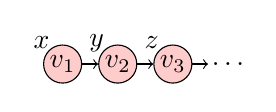
\begin{tikzpicture}[baseline,node distance=7mm, yshift=2pt, every
    node/.style={fill=red!20,circle,draw,inner sep=1pt}]
  \node (x) {$v_1$};
  \node[right of=x] (y) {$v_2$};
  \node[right of=y] (z) {$v_3$};
  \node[right of=z,draw=none,fill=none] (dots) {$\ldots$};
  \node[above left of=x,node distance=3.8mm,draw=none,fill=none] {$x$};
  \node[above left of=y,node distance=3.8mm,draw=none,fill=none] {$y$};
  \node[above left of=z,node distance=3.8mm,draw=none,fill=none] {$z$};
  \path[->] (x) edge (y);
  \path[->] (y) edge (z);
  \path[->] (z) edge (dots);
\end{tikzpicture}
* \displaystyle{\iterStar_{(x,y)\notin S}
  \iterStar_{v} [\text{U}(x,y,v)]
  * \iterStar_{(x,y)\in S}
  \exsts{w}\iterStar_{v\neq w} [\text{U}(x,y,v)]}}
{I_x \cup I_y\cup I_z\cup \cdots}{s}
\]
%
%{\centering 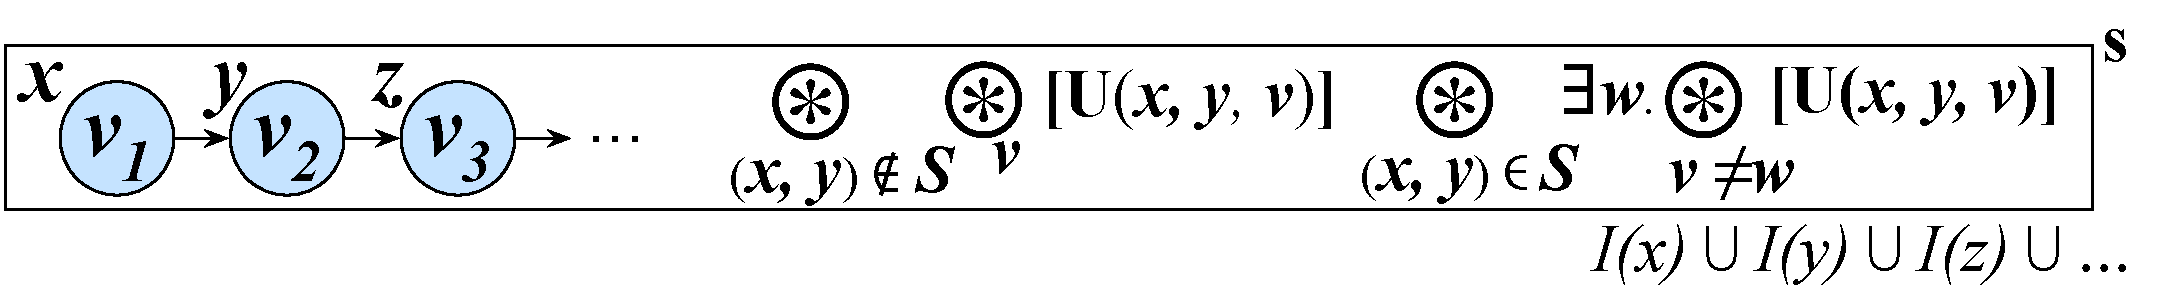
\includegraphics[scale=0.232]{Sections/Examples/Images/capSet.pdf}\\}
%
%
The set is represented as a sorted singly-linked list with no
duplicate elements. The list starts at address $x$ with value $v_1$,
points to the next element at address $y$ with value $v_2$, and so
forth. Hereafter, we write $\node{x}{v}{y}$ to denote a node at
address $x$, with value $v$ and successor $y$. 

All nodes of the list reside in a single shared region labelled $s$ and the interference on the list is the combined interference associated with each constituent node. 
Each node at a given address $x$ is associated with a set of update capabilities of the form $[\text{U}(x, y, v)]$ for \emph{all} possible addresses $y$ and \emph{all} possible values $v$. This is to capture all potential successor addresses $y$ and all potential values $v$ that may be stored at address $x$. 
%For instance, since the value $v_{1}$ may be contained in the list at address $x$ before address $y$, there must exist an update capability $[\text{U}(x, y, v_1)]$ to accommodate possible modifications of value $v_{1}$ with respect to $x$ and $y$. 
In order to modify a node, a thread can acquire the lock associated with the node and subsequently claim the relevant update capability.
% 

Since in CAP the capabilities associated with a region can only be generated upon its creation, the shared region is required to keep track of all possible update capabilities $[\text{U}(x, y, v)]$ associated with all addresses $x$ (including those not currently in the domain of the list), all addresses $y$ and all values $v$. At any one point, given $\node{x}{v}{y}$, the only update capability that can be claimed by a thread (through locking) is the one that reflects its current status, namely $[\text{U}(x, y, v)]$. As a result, an auxiliary mathematical set $S$ is used to track those nodes of the list that are currently locked and thus infer which $[\text{U}]$ capabilities have been claimed. The distribution of update capabilities is captured by the two assertions written as the \emph{infinite multiplicative star operator} $\iterStar$. The first part of the assertion states that given any node at address $x$ with successor $y$, if it is not locked, i.e.\ $(x, y) \not\in S$, then {all} of its update capabilities of the form $[\text{U}(x, y, v)]$ lie in the shared region for {all} values $v$. Dually, if it is locked, i.e.\ $(x, y) \in S$, then the update capabilities for {all} values $v$ {but one} ($w \not= v$) are in the shared region.

This CAP set predicate is unnecessarily complicated. It is counter-intuitive
to have to  account for the capabilities associated with   addresses not in the domain of the list. Moreover, each thread observes all nodes in the list and thus needs to account for their associated interference. 

TaDA~\cite{tada} took the first steps towards addressing the above
shortcomings of the CAP approach. TaDA regions are parametric in the
separation algebra of capabilities (called guards).
As such, one can choose a
more suitable algebra to axiomatise the desired behaviour of capabilities. 
%It can  therefore
%provide  a set region which just
%describes the elements of a set. This region  can grow and decrease using
%capabilities and axioms on regions. 
%For instance, when creating the set region $r$, one can choose a capability algebra that satisfies the following axiom.\vspace{-7pt}
%%
%\begin{align*}
%	[\textsc{S}(vs)]_r <=> [\textsc{S}(vs\uplus\{v\})]_r * [\textsc{U}(v)]_r   \\[-20pt]
%\end{align*}
%%
%This axiom effectively ensures that when the set region $r$ contains values $vs$, it may be extended with value $v$, and in doing so claim the the accompanying update capability $[\text{U}(v)]_r$. 
While TaDA's approach is much cleaner than that of CAP, it nevertheless requires the foresight of specifying all desired interference associated with the region upon its creation. 
As such, interference specifications are \emph{static} and cannot be extended with new behaviour even when the existing resources are left untouched. 
On the other hand, as well as being parametric in its capability
separation algebra, the dynamic subjective views of \colosl provide
local reasoning about  the shared resource and its interference. 
%

We proceed with the \colosl proof of the set implementation. Recall from \S\ref{sec:colosl} that \colosl is parametric in the separation algebra of capabilities. We thus instantiate it with a heap-like capability separation algebra that is \emph{stateful} and demonstrate that this allows for a more concise proof.  

We specify the set predicate as the $*$-composition of  subjective
views associated  each node in the singly-linked list as illustrated
by:

{\centering
\begin{tikzpicture}
  \node[inner sep=0pt,outer sep=0pt] (xNy) {$[\nextC{x}{y}] *\null$};
  \node[right of=xNy,circle,draw,fill=blue!15,inner sep=1pt,xshift=2pt] (v1) {$v_1$};
  \node[above left of=v1,node distance=3.8mm,draw=none,fill=none,inner sep=0pt,outer sep=1pt] (x) {$x$};
  \node[fit=(xNy) (v1) (x),rounded corners,rectangle,draw,inner sep=1pt] (n1) {};
  \node[right of=n1, anchor=north west,xshift=0ex] {$I_x$};

  \node[right of=n1,xshift=2.5ex] {$*$};

  \node[inner sep=0pt,outer sep=0pt,right of=xNy,node distance=2.7cm] (yNz) {$[\nextC{y}{z}] *\null$};
  \node[right of=yNz,circle,draw,fill=blue!15,inner sep=1pt,xshift=2pt] (v2) {$v_2$};
  \node[above left of=v2,node distance=3.8mm,draw=none,fill=none,inner sep=0pt,outer sep=0pt] (y) {$y$};
  \node[fit=(yNz) (v2) (y),rounded corners,rectangle,draw,inner sep=1pt] (n2) {};
  \node[right of=n2, anchor=north west,xshift=0ex] {$I_y$};
  \node[right of=n2,xshift=2.5ex] {$*$};

  \node[inner sep=0pt,outer sep=0pt,right of=yNz,node distance=2.9cm] (zN) {$[\nextC{z}{\dots}] *\null$};
  \node[right of=zN,circle,draw,fill=blue!15,inner sep=1pt,xshift=5pt] (v3) {$v_3$};
  \node[above left of=v3,node distance=3.8mm,draw=none,fill=none,inner sep=0pt,outer sep=1pt] (z) {$z$};
  \node[fit=(zN) (v3) (z),rounded corners,rectangle,draw,inner sep=1pt] (n3) {};
  \node[right of=n3, anchor=north west,xshift=1ex] {$I_z$};
  \node[right of=n3,xshift=3.5ex] {$*$};

  \node[inner sep=0pt,outer sep=0pt,right of=zN,node distance=2.3cm] (dots) {$\cdots$};

  \path[->] (v1.north east) edge[semithick,bend left=55] (n2.west);
  \path[->] (v2.north east) edge[semithick,bend left=55] (n3.west);
  \path[->] (v3.north east) edge[semithick,bend left=55] (dots.north west);
\end{tikzpicture}\\}
\noindent  The interference on each subjective view is limited to the
node in question. Associated with each node at address $x$ is a
``next'' capability $[\nextC{x}{y}]$ that tracks its successor
$y$. This is analogous to the $[\text{U}(x, y, v)]$ capability of CAP
and we shortly demonstrate how it is utilised in our reasoning. 

Since \colosl allows for {dynamic} extension of the shared state, we do not need to account for capabilities associated with all addresses. Instead, fresh capabilities are generated dynamically as needed. We demonstrate this by giving a reasoning outline of the \li{add(}$v'$\li{)} method that adds value $v'$ to the set by inserting it in the sorted list.
Suppose $v_2 < v' < v_3$, and thus a new node $w$ with value $v'$ is
to be inserted after node $y$.  The operating thread proceeds by
traversing the list by hand-over-hand locking until it reaches node
$y$. It then locks $y$ and claims its next pointer and moves it to its
local state, as allowed by $I_y$. Subsequently, the shared state is
{extended} by the resources associated with the new node and its
associated capabilities ($[\nextC{w}{z}]$) are generated on the fly as
illustrated by:\vspace{0pt}

{\centering
\begin{tikzpicture}
  \node[inner sep=0pt,outer sep=0pt] (xNy) {$[\nextC{x}{y}] *\null$};
  \node[right of=xNy,circle,draw,fill=blue!15,inner sep=1pt,xshift=2pt] (v1) {$v_1$};
  \node[above left of=v1,node distance=3.8mm,draw=none,fill=none,inner sep=0pt,outer sep=1pt] (x) {$x$};
  \node[fit=(xNy) (v1) (x),rounded corners,rectangle,draw,inner sep=1pt] (n1) {};
  \node[right of=n1, anchor=north west,xshift=0ex] {$I_x$};

  \node[right of=xNy,node distance=1.7cm] {$*$};

  \node[inner sep=0pt,outer sep=0pt,right of=xNy,node distance=2.7cm] (yNz) {$[\nextC{y}{z}] *\null$};
  \node[right of=yNz,circle,draw,fill=blue!15,inner sep=1pt,xshift=2pt] (v2) {$v_2$};
  \node[above left of=v2,node distance=3.8mm,draw=none,fill=none,inner sep=0pt,outer sep=0pt] (y) {$y$};
  \node[fit=(yNz) (v2) (y),rounded corners,rectangle,draw,inner sep=1pt] (n2) {};
  \node[right of=n2, anchor=north west,xshift=0ex] {$I_y$};
  \node[right of=yNz,node distance=1.7cm] {$*$};

  \node[inner sep=0pt,outer sep=0pt,right of=yNz,node distance=2.7cm] (wNz) {$[\nextC{w}{{\color{red}z}}] *\null$};
  \node[right of=wNz,circle,draw,fill=blue!15,inner sep=1pt,xshift=2pt] (v4) {$v'$};
  \node[above left of=v4,node distance=3.8mm,draw=none,fill=none,inner sep=0pt,outer sep=1pt] (w) {$w$};
  \node[fit=(wNz) (v4) (w),rounded corners,rectangle,draw,inner sep=1pt] (n4) {};
  \node[right of=n4, anchor=north west,xshift=0.4ex] {$I_w$};
  \node[right of=wNz,node distance=1.75cm] {$*$};

  \node[inner sep=0pt,outer sep=0pt,right of=wNz,node distance=2.9cm] (zN) {$[\nextC{z}{\dots}] *\null$};
  \node[right of=zN,circle,draw,fill=blue!15,inner sep=1pt,xshift=5pt] (v3) {$v_3$};
  \node[above left of=v3,node distance=3.8mm,draw=none,fill=none,inner sep=0pt,outer sep=1pt] (z) {$z$};
  \node[fit=(zN) (v3) (z),rounded corners,rectangle,draw,inner sep=1pt] (n5) {};
  \node[right of=n5, anchor=north west,xshift=1ex] {$I_z$};
  \node[right of=zN,node distance=1.8cm] {$*$};

  \node[inner sep=0pt,outer sep=0pt,right of=zN,node distance=2.3cm] (dots) {$\cdots$};

  \draw[fill=red,semithick] (v2.north east) + (-2pt,-2pt)  rectangle +(2pt,2pt);
  \draw[semithick] (v2.north east) + (2pt,2pt) arc (0:180:2pt);  
  \path[->] (v1.north east) edge[semithick,bend left=55] (n2.west);
  \path[->] (v3.north east) edge[semithick,bend left=55] (dots.north west);
  \path[->] (v4.north east) edge[semithick,bend left=55,red] (n5.west);
\end{tikzpicture}\\}
%
%{\centering 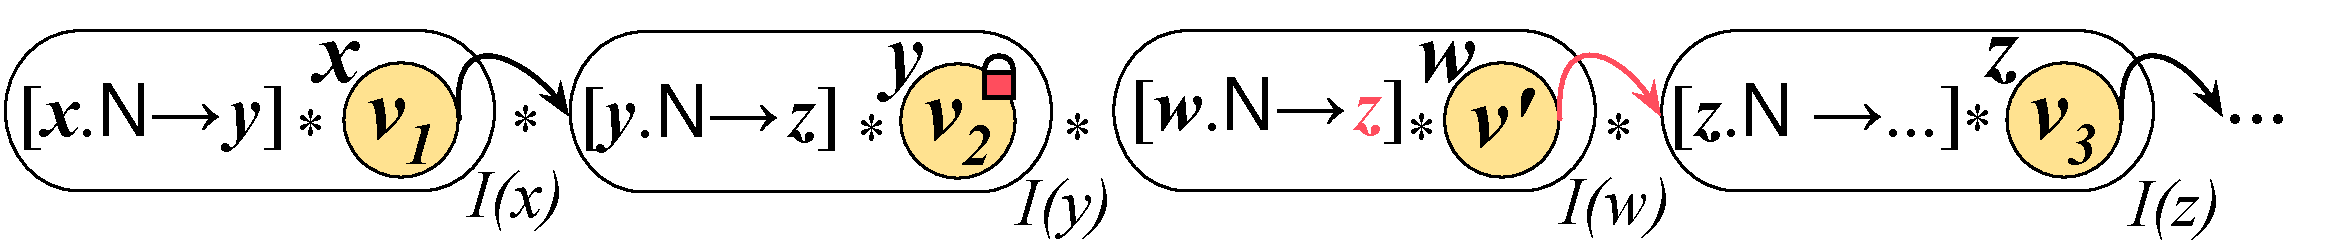
\includegraphics[scale=0.25]{Sections/Examples/Images/add1.pdf}\\}
%
%At this point, since the locking thread holds the next pointer of $y$ in its local state, it modifies it to point to the new node $w$. It then unlocks $y$ and returns its next pointer to the shared state. However, the interference assertion associated with node $y$ ($I_y$) allows the node to be unlocked in three possible ways. Either its successor has not changed from its old value $z$ (tracked by $\nextC{y}{z}$); \emph{or} it has been redirected to $z$'s successor (when $z$ is being deleted); \emph{or} it has been directed to a new node whose successor is $z$ (a new node is inserted between $y$ and $z$). When adding a new node after $y$, the latter of the possibilities is applicable and thus the unlocking thread must demonstrate that the new node ($w$) does indeed point to $z$. In order to establish this condition, we use the (\mergeRule) principle in our reasoning to combine the subjective views of $y$ and $w$ as follows.
\noindent Since the locking thread holds the next pointer of $y$ in
its local state, it modifies it to point to the new node $w$. It then
unlocks $y$ and returns its next pointer to the shared state. When
inserting a new node between $y$ and $z$, the associated interference
assertion $I_y$ allows $y$ to be unlocked only if it has been directed
to a new node whose successor is $z$. As such, the unlocking thread
must demonstrate that the new node $w$ does indeed point to $z$. In
order to establish this, we use the \mergeRule principle to combine
the subjective views of $y$ and $w$ as follows: \vspace{0pt}

{\centering
\begin{tikzpicture}
  \node[inner sep=0pt,outer sep=0pt] (xNy) {$[\nextC{x}{y}] *\null$};
  \node[right of=xNy,circle,draw,fill=blue!15,inner sep=1pt,xshift=2pt] (v1) {$v_1$};
  \node[above left of=v1,node distance=3.8mm,draw=none,fill=none,inner sep=0pt,outer sep=1pt] (x) {$x$};
  \node[fit=(xNy) (v1) (x),rounded corners,rectangle,draw,inner sep=1pt] (n1) {};
  \node[right of=n1, anchor=north west,xshift=0ex] {$I_x$};

  \node[right of=xNy,node distance=1.7cm] {$*$};

  \node[inner sep=0pt,outer sep=0pt,right of=xNy,node distance=2.7cm] (yNz) {$[\nextC{y}{z}] *\null$};
  \node[right of=yNz,circle,draw,fill=blue!15,inner sep=1pt,xshift=2pt] (v2) {$v_2$};
  \node[above left of=v2,node distance=3.8mm,draw=none,fill=none,inner sep=0pt,outer sep=0pt] (y) {$y$};

  \node[inner sep=0pt,outer sep=0pt,right of=v2,node distance=1.25cm] (wNz) {$\null*[\nextC{w}{z}] *\null$};
  \node[right of=wNz,circle,draw,fill=blue!15,inner sep=1pt,xshift=7pt] (v4) {$v'$};
  \node[above left of=v4,node distance=3.8mm,draw=none,fill=none,inner sep=0pt,outer sep=1pt] (w) {$w$};
  \node[fit=(wNz) (v4) (w) (yNz) (v2) (y),rounded corners,rectangle,draw,inner sep=1pt] (n4) {};
  \node[right of=n4, anchor=north west,xshift=8.4ex] {$I_y\cup I_w$};
  \node[right of=wNz,node distance=2.6cm] {$*$};

  \node[inner sep=0pt,outer sep=0pt,right of=wNz,node distance=3.8cm] (zN) {$[\nextC{z}{\dots}] *\null$};
  \node[right of=zN,circle,draw,fill=blue!15,inner sep=1pt,xshift=5pt] (v3) {$v_3$};
  \node[above left of=v3,node distance=3.8mm,draw=none,fill=none,inner sep=0pt,outer sep=1pt] (z) {$z$};
  \node[fit=(zN) (v3) (z),rounded corners,rectangle,draw,inner sep=1pt] (n5) {};
  \node[right of=n5, anchor=north west,xshift=1ex] {$I_z$};
  \node[right of=zN,node distance=1.8cm] {$*$};

  \node[inner sep=0pt,outer sep=0pt,right of=zN,node distance=2.3cm] (dots) {$\cdots$};

  \draw[fill=red,semithick] (v2.north east) + (-2pt,-2pt)  rectangle +(2pt,2pt);
  \draw[semithick] (v2.north east) + (2pt,2pt) arc (0:180:2pt);  
  \path[->] (v1.north east) edge[semithick,bend left=55] (n2.west);
  \path[->] (v3.north east) edge[semithick,bend left=55] (dots.north west);
  \path[->] (v4.north east) edge[semithick,bend left=55] (n5.west);
\end{tikzpicture}\\}
%
%x{\centering 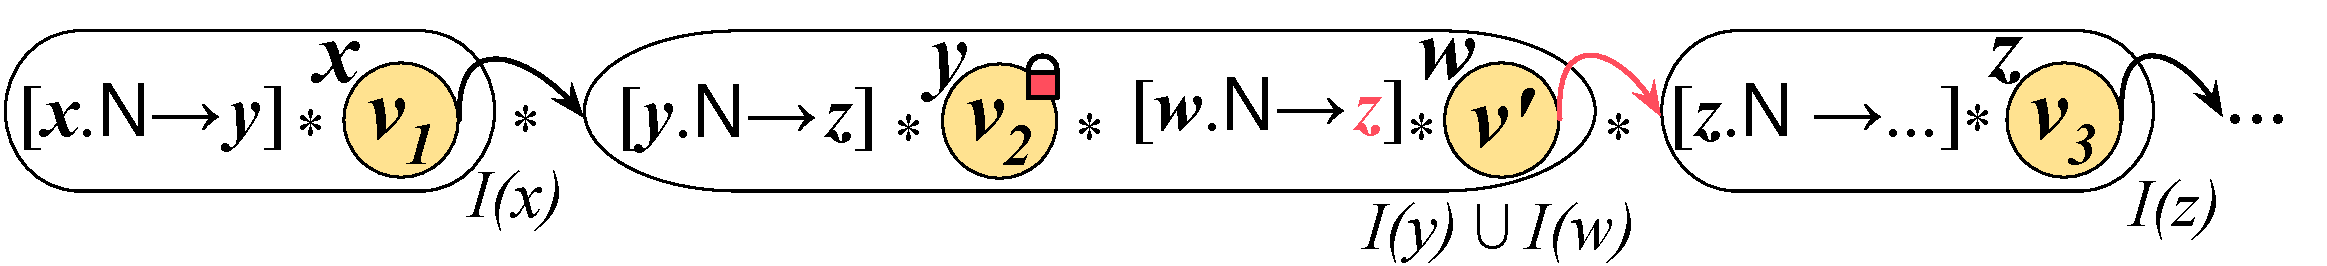
\includegraphics[scale=0.25]{Sections/Examples/Images/add2.pdf}\\}
%
%Finally, node $y$ is unlocked; its updated next pointer is returned to the shared state and its next capability is modified accordingly to reflect its new successor. Using the (\copyRule), (\forgetRule) and (\shiftRule) principles \textit{ad seriatim}, we can once again obtain the set predicate with the new node $w$ inserted. 
\noindent Finally, $y$ is unlocked; its next pointer is returned to the shared state and its next capability is modified to reflect its new successor. Using the \copyRule, \forgetRule and \shiftRule principles in order, we obtain the set predicate with $w$ inserted. \vspace{0pt}

{\centering
\begin{tikzpicture}
  \node[inner sep=0pt,outer sep=0pt] (xNy) {$[\nextC{x}{y}] *\null$};
  \node[right of=xNy,circle,draw,fill=blue!15,inner sep=1pt,xshift=2pt] (v1) {$v_1$};
  \node[above left of=v1,node distance=3.8mm,draw=none,fill=none,inner sep=0pt,outer sep=1pt] (x) {$x$};
  \node[fit=(xNy) (v1) (x),rounded corners,rectangle,draw,inner sep=1pt] (n1) {};
  \node[right of=n1, anchor=north west,xshift=0ex] {$I_x$};

  \node[right of=xNy,node distance=1.7cm] {$*$};

  \node[inner sep=0pt,outer sep=0pt,right of=xNy,node distance=2.7cm] (yNz) {$[\nextC{y}{{\color{red}w}}] *\null$};
  \node[right of=yNz,circle,draw,fill=blue!15,inner sep=1pt,xshift=2pt] (v2) {$v_2$};
  \node[above left of=v2,node distance=3.8mm,draw=none,fill=none,inner sep=0pt,outer sep=0pt] (y) {$y$};
  \node[fit=(yNz) (v2) (y),rounded corners,rectangle,draw,inner sep=1pt] (n2) {};
  \node[right of=n2, anchor=north west,xshift=0ex] {$I_y$};
  \node[right of=yNz,node distance=1.7cm] {$*$};

  \node[inner sep=0pt,outer sep=0pt,right of=yNz,node distance=2.7cm] (wNz) {$[\nextC{w}{z}] *\null$};
  \node[right of=wNz,circle,draw,fill=blue!15,inner sep=1pt,xshift=2pt] (v4) {$v'$};
  \node[above left of=v4,node distance=3.8mm,draw=none,fill=none,inner sep=0pt,outer sep=1pt] (w) {$w$};
  \node[fit=(wNz) (v4) (w),rounded corners,rectangle,draw,inner sep=1pt] (n4) {};
  \node[right of=n4, anchor=north west,xshift=0.4ex] {$I_w$};
  \node[right of=wNz,node distance=1.75cm] {$*$};

  \node[inner sep=0pt,outer sep=0pt,right of=wNz,node distance=2.9cm] (zN) {$[\nextC{z}{\dots}] *\null$};
  \node[right of=zN,circle,draw,fill=blue!15,inner sep=1pt,xshift=5pt] (v3) {$v_3$};
  \node[above left of=v3,node distance=3.8mm,draw=none,fill=none,inner sep=0pt,outer sep=1pt] (z) {$z$};
  \node[fit=(zN) (v3) (z),rounded corners,rectangle,draw,inner sep=1pt] (n5) {};
  \node[right of=n5, anchor=north west,xshift=1ex] {$I_z$};
  \node[right of=zN,node distance=1.8cm] {$*$};

  \node[inner sep=0pt,outer sep=0pt,right of=zN,node distance=2.3cm] (dots) {$\cdots$};

  \path[->] (v1.north east) edge[semithick,bend left=55] (n2.west);
  \path[->] (v2.north east) edge[semithick,bend left=55,red] (n4.west);
  \path[->] (v3.north east) edge[semithick,bend left=55] (dots.north west);
  \path[->] (v4.north east) edge[semithick,bend left=55] (n5.west);
\end{tikzpicture}\\}
%
%{\centering 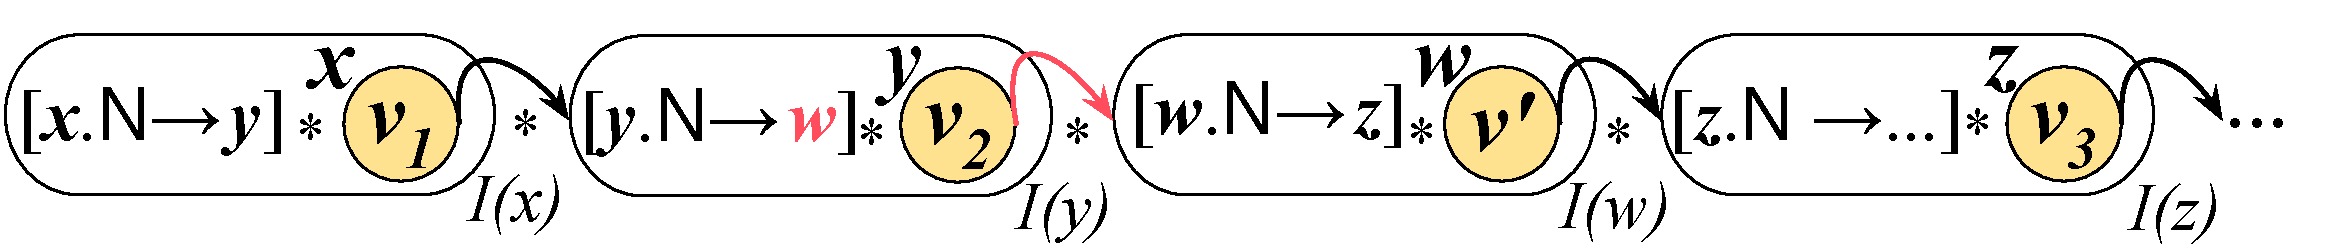
\includegraphics[scale=0.25]{Sections/Examples/Images/add3.pdf}\\}
%
We can reason about the \li{remove} operation in a similar
fashion. The dynamic extension afforded by the \extendRule\ principle
allows us to generate new capabilities only when needed and thus gives
way to a concise proof. 
%
Moreover, rather than having a distinct capability to modify the element at address $x$, for each possible successor address $y$ (as with $[\text{U}(x, y, v)]$ in CAP), we appeal to a single capability of the form $[\nextC{x}{y}]$ that is modified to $[\nextC{x}{y'}]$ whenever $x$'s successor changes from $y$ to $y'$.
%the capability is modified accordingly to record the changes to the successor address. 
%
Lastly, using the reasoning principles of \mergeRule, \forgetRule,
\shiftRule\ and \copyRule, we can grow and shrink our subjective views
as needed. This means that,  at any one point, we only view the relevant parts of the shared state. 
%
The technical details can be found in~\cite{colosl-tr14}. 
